%  LaTeX support: latex@mdpi.com 
%  For support, please attach all files needed for compiling as well as the log file, and specify your operating system, LaTeX version, and LaTeX editor.

%=================================================================
\documentclass[journal,article,submit,pdftex,moreauthors]{Definitions/mdpi} 
\usepackage{subfig}
\usepackage[textsize=small]{todonotes}
\newcommand{\ie}{\textit{i.~e.} }
\newcommand{\cref}{c^{\ominus}}
%\newcommand{\cs}{c_{s}}
\newcommand{\kT}{k_\mathrm{B}T}
\newcommand{\kB}{k_\mathrm{B}}
\newcommand{\lb}{l_\mathrm{B}}
%\newcommand{\NA}{N_{\mathrm{A^-}}}
\newcommand{\NA}{N_{\mathrm{A}}}
\newcommand{\muna}{\mu_\mathrm{Na^+}}

\newcommand{\mucl}{\mu_\mathrm{Cl^-}}
\newcommand{\muca}{\mu_\mathrm{Ca^{2+}}}
\newcommand{\muh}{\mu_\mathrm{H^+}}
\newcommand{\mua}{\mu_\mathrm{A^-}}
\newcommand{\muha}{\mu_\mathrm{HA}}
\newcommand{\muoh}{\mu_\mathrm{OH}}

\newcommand{\cna}{c_\mathrm{Na^+}}
\newcommand{\ccl}{c_\mathrm{Cl^-}}
\newcommand{\cca}{c_\mathrm{Ca^{2+}}}
\newcommand{\ch}{c_\mathrm{H^+}}
\newcommand{\cp}{c_\mathrm{p}}
\newcommand{\nna}{n_\mathrm{Na^+}}
\newcommand{\ncl}{n_\mathrm{Cl^-}}
\newcommand{\Nna}{N_\mathrm{Na^+}}
\newcommand{\Ncl}{N_\mathrm{Cl^-}}

\newcommand{\ncleq}{\widetilde{N}_\mathrm{Cl^-}}
\newcommand{\nca}{N_\mathrm{Ca^{2+}}}

\newcommand{\superin}{^\mathrm{in}}
\newcommand{\subin}{_\mathrm{in}}
\newcommand{\subi}{_\mathrm{i}}

\newcommand{\gel}{^\mathrm{gel}}
\newcommand{\tot}{^\mathrm{tot}}
\newcommand{\out}{^{\mathrm{out}}}
\newcommand{\coh}{c_\mathrm{OH}}
\newcommand{\bulk}{^{\mathrm{b}}}
\renewcommand{\H}{\mathrm{H^+}}
\newcommand{\A}{\mathrm{A^-}}
\newcommand{\AH}{\mathrm{AH}}
%%%%%%%%%%%%%%%%%%%%%%%%%%%%%% LyX specific LaTeX commands.

\newcommand{\cl}{\mathrm{Cl^-}}
\newcommand{\br}{\mathrm{Br^-}}
\newcommand{\na}{\mathrm{Na^+}}
\newcommand{\h}{\mathrm{H^+}}
\newcommand{\ka}{\mathrm{K^+}}
\newcommand{\oh}{\mathrm{OH^-}}
\newcommand{\ca}{\mathrm{Ca^{2+}}}
\newcommand{\mg}{\mathrm{Mg^{2+}}}

\newcommand{\Ka}{K_{\mathrm{A}}}
\newcommand{\pKa}{\mathrm{p}\Ka}
\newcommand{\pK}{\mathrm{p}K}
\newcommand{\pH}{\mathrm{pH}}
\newcommand{\mol}{\mathrm{mol}}
\newcommand{\molperl}{\mathrm{mol/l}}
\newcommand{\kg}{\mathrm{kg}}
\newcommand{\res}{^{\mathrm{res}}}
\newcommand{\pHres}{\pH\res}
\newcommand{\pHgel}{\pH\gel}
\newcommand{\cs}{c_{\mathrm{s}}}
%\newcommand{\cs}{c_{\mathrm{salt}}}
\newcommand{\csres}{\cs\res}
%\newcommand{\Vgel}{V\gel}
\newcommand{\Vgel}{V_\mathrm{gel}}
%\newcommand{\Vgel}{V}
\newcommand{\Ngel}{N_\mathrm{gel}}
%\newcommand{\Vgeleq}{\widetilde{V}_\mathrm{gel}}}
%\newcommand{\Pgel}{P_\mathrm{gel}}
\newcommand{\Pgel}{\Pi}
\newcommand{\Pres}{P_\mathrm{res}}
\newcommand{\Pout}{P_\mathrm{out}}
\newcommand{\Vout}{V_\mathrm{out}}
%\newcommand{\Vbox}{V_\mathrm{box}}
\newcommand{\Vbox}{V_0}
\newcommand{\PE}{polyelectrolyte{}}

\newcommand{\reffig}[1]{Figure~\ref{#1}}
\newcommand{\refeq}[1]{Equation~\ref{#1}{}}
\newcommand{\etal}{\textit{et al.}{}}

% For posting an early version of this manuscript as a preprint, you may use "preprints" as the journal and change "submit" to "accept". The document class line would be, e.g., \documentclass[preprints,article,accept,moreauthors,pdftex]{mdpi}. This is especially recommended for submission to arXiv, where line numbers should be removed before posting. For preprints.org, the editorial staff will make this change immediately prior to posting.

%--------------------
% Class Options:
%--------------------
%----------
% journal
%----------
% Choose between the following MDPI journals:
% acoustics, actuators, addictions, admsci, adolescents, aerospace, agriculture, agriengineering, agronomy, ai, algorithms, allergies, alloys, analytica, animals, antibiotics, antibodies, antioxidants, applbiosci, appliedchem, appliedmath, applmech, applmicrobiol, applnano, applsci, aquacj, architecture, arts, asc, asi, astronomy, atmosphere, atoms, audiolres, automation, axioms, bacteria, batteries, bdcc, behavsci, beverages, biochem, bioengineering, biologics, biology, biomass, biomechanics, biomed, biomedicines, biomedinformatics, biomimetics, biomolecules, biophysica, biosensors, biotech, birds, bloods, blsf, brainsci, breath, buildings, businesses, cancers, carbon, cardiogenetics, catalysts, cells, ceramics, challenges, chemengineering, chemistry, chemosensors, chemproc, children, chips, cimb, civileng, cleantechnol, climate, clinpract, clockssleep, cmd, coasts, coatings, colloids, colorants, commodities, compounds, computation, computers, condensedmatter, conservation, constrmater, cosmetics, covid, crops, cryptography, crystals, csmf, ctn, curroncol, currophthalmol, cyber, dairy, data, dentistry, dermato, dermatopathology, designs, diabetology, diagnostics, dietetics, digital, disabilities, diseases, diversity, dna, drones, dynamics, earth, ebj, ecologies, econometrics, economies, education, ejihpe, electricity, electrochem, electronicmat, electronics, encyclopedia, endocrines, energies, eng, engproc, ent, entomology, entropy, environments, environsciproc, epidemiologia, epigenomes, est, fermentation, fibers, fintech, fire, fishes, fluids, foods, forecasting, forensicsci, forests, foundations, fractalfract, fuels, futureinternet, futureparasites, futurepharmacol, futurephys, futuretransp, galaxies, games, gases, gastroent, gastrointestdisord, gels, genealogy, genes, geographies, geohazards, geomatics, geosciences, geotechnics, geriatrics, hazardousmatters, healthcare, hearts, hemato, heritage, highthroughput, histories, horticulturae, humanities, humans, hydrobiology, hydrogen, hydrology, hygiene, idr, ijerph, ijfs, ijgi, ijms, ijns, ijtm, ijtpp, immuno, informatics, information, infrastructures, inorganics, insects, instruments, inventions, iot, j, jal, jcdd, jcm, jcp, jcs, jdb, jeta, jfb, jfmk, jimaging, jintelligence, jlpea, jmmp, jmp, jmse, jne, jnt, jof, joitmc, jor, journalmedia, jox, jpm, jrfm, jsan, jtaer, jzbg, kidney, kidneydial, knowledge, land, languages, laws, life, liquids, literature, livers, logics, logistics, lubricants, lymphatics, machines, macromol, magnetism, magnetochemistry, make, marinedrugs, materials, materproc, mathematics, mca, measurements, medicina, medicines, medsci, membranes, merits, metabolites, metals, meteorology, methane, metrology, micro, microarrays, microbiolres, micromachines, microorganisms, microplastics, minerals, mining, modelling, molbank, molecules, mps, msf, mti, muscles, nanoenergyadv, nanomanufacturing, nanomaterials, ncrna, network, neuroglia, neurolint, neurosci, nitrogen, notspecified, nri, nursrep, nutraceuticals, nutrients, obesities, oceans, ohbm, onco, oncopathology, optics, oral, organics, organoids, osteology, oxygen, parasites, parasitologia, particles, pathogens, pathophysiology, pediatrrep, pharmaceuticals, pharmaceutics, pharmacoepidemiology, pharmacy, philosophies, photochem, photonics, phycology, physchem, physics, physiologia, plants, plasma, pollutants, polymers, polysaccharides, poultry, powders, preprints, proceedings, processes, prosthesis, proteomes, psf, psych, psychiatryint, psychoactives, publications, quantumrep, quaternary, qubs, radiation, reactions, recycling, regeneration, religions, remotesensing, reports, reprodmed, resources, rheumato, risks, robotics, ruminants, safety, sci, scipharm, seeds, sensors, separations, sexes, signals, sinusitis, skins, smartcities, sna, societies, socsci, software, soilsystems, solar, solids, sports, standards, stats, stresses, surfaces, surgeries, suschem, sustainability, symmetry, synbio, systems, taxonomy, technologies, telecom, test, textiles, thalassrep, thermo, tomography, tourismhosp, toxics, toxins, transplantology, transportation, traumacare, traumas, tropicalmed, universe, urbansci, uro, vaccines, vehicles, venereology, vetsci, vibration, viruses, vision, waste, water, wem, wevj, wind, women, world, youth, zoonoticdis 

%---------
% article
%---------
% The default type of manuscript is "article", but can be replaced by: 
% abstract, addendum, article, book, bookreview, briefreport, casereport, comment, commentary, communication, conferenceproceedings, correction, conferencereport, entry, expressionofconcern, extendedabstract, datadescriptor, editorial, essay, erratum, hypothesis, interestingimage, obituary, opinion, projectreport, reply, retraction, review, perspective, protocol, shortnote, studyprotocol, systematicreview, supfile, technicalnote, viewpoint, guidelines, registeredreport, tutorial
% supfile = supplementary materials

%----------
% submit
%----------
% The class option "submit" will be changed to "accept" by the Editorial Office when the paper is accepted. This will only make changes to the frontpage (e.g., the logo of the journal will get visible), the headings, and the copyright information. Also, line numbering will be removed. Journal info and pagination for accepted papers will also be assigned by the Editorial Office.

%------------------
% moreauthors
%------------------
% If there is only one author the class option oneauthor should be used. Otherwise use the class option moreauthors.

%---------
% pdftex
%---------
% The option pdftex is for use with pdfLaTeX. If eps figures are used, remove the option pdftex and use LaTeX and dvi2pdf.

%=================================================================
% MDPI internal commands
\firstpage{1} 
\makeatletter 
\setcounter{page}{\@firstpage} 
\makeatother
\pubvolume{1}
\issuenum{1}
\articlenumber{0}
\pubyear{2022}
\copyrightyear{2022}
%\externaleditor{Academic Editor: Firstname Lastname}
\datereceived{} 
%\daterevised{} % Only for the journal Acoustics
\dateaccepted{} 
\datepublished{} 
%\datecorrected{} % Corrected papers include a "Corrected: XXX" date in the original paper.
%\dateretracted{} % Corrected papers include a "Retracted: XXX" date in the original paper.
\hreflink{https://doi.org/} % If needed use \linebreak
%\doinum{}
%------------------------------------------------------------------
% The following line should be uncommented if the LaTeX file is uploaded to arXiv.org
%\pdfoutput=1

%=================================================================
% Add packages and commands here. The following packages are loaded in our class file: fontenc, inputenc, calc, indentfirst, fancyhdr, graphicx, epstopdf, lastpage, ifthen, lineno, float, amsmath, setspace, enumitem, mathpazo, booktabs, titlesec, etoolbox, tabto, xcolor, soul, multirow, microtype, tikz, totcount, changepage, attrib, upgreek, cleveref, amsthm, hyphenat, natbib, hyperref, footmisc, url, geometry, newfloat, caption

%=================================================================
%% Please use the following mathematics environments: Theorem, Lemma, Corollary, Proposition, Characterization, Property, Problem, Example, ExamplesandDefinitions, Hypothesis, Remark, Definition, Notation, Assumption
%% For proofs, please use the proof environment (the amsthm package is loaded by the MDPI class).

%=================================================================
% Full title of the paper (Capitalized)
%\Title{Water desalination using polyelectrolyte hydrogel. Gibbs ensemble modeling}
\Title{Water desalination using polyelectrolyte hydrogel: Gibbs ensemble modeling}

% Alternative titles
%\Title{What the Gibbs ensemble modeling says about water desalination using polyelectrolyte hydrogel}
%\Title{Water desalination using polyelectrolyte hydrogel from the Gibbs ensemble modeling point of view}



% MDPI internal command: Title for citation in the left column
\TitleCitation{Title}

% Author Orchid ID: enter ID or remove command
\newcommand{\orcidauthorA}{0000-0003-3412-7707} % Add \orcidA{} behind the author's name
\newcommand{\orcidauthorB}{0000-0003-3616-3285} % Add \orcidB{} behind the author's name
\newcommand{\orcidauthorC}{0000-0002-8501-0464} % Add \orcidB{} behind the author's name

% Authors, for the paper (add full first names)
\Author{Mikhail Laktionov $^{1, 2}$\orcidA{}, Lucie Nová $^{1}$\orcidB{} and Oleg V. Rud $^{1, 3}$*\orcidC{}}

\keyword{polyelectrolye hydrogel; simulation; desalination} 
%\longauthorlist{yes}

% MDPI internal command: Authors, for metadata in PDF
\AuthorNames{Mikhail Laktionov, Lucie Nová and Oleg V. Rud}

% MDPI internal command: Authors, for citation in the left column
\AuthorCitation{Lastname, F.; Lastname, F.; Lastname, F.}
% If this is a Chicago style journal: Lastname, Firstname, Firstname Lastname, and Firstname Lastname.

% Affiliations / Addresses (Add [1] after \address if there is only one affiliation.)
\address{%
$^{1}$ \quad Department of Physical and Macromolecular Chemistry, Faculty of Science, Charles University in Prague, Czech Republic; e-mail@e-mail.com\\
$^{2}$ \quad St. Petersburg National Research University of Information Technologies, Mechanics and Optics, St. Petersburg, Russia; e-mail@e-mail.com\\
$^{3}$ \quad Institute of Macromolecular Compounds of Russian Academy of Sciences, Saint-Petersburg, Russia; e-mail@e-mail.com}


% Contact information of the corresponding author
\corres{Correspondence: oleg.rud@natur.cuni.cz; }

% Current address and/or shared authorship
%\firstnote{Current address: Affiliation 3.} 
%\secondnote{These authors contributed equally to this work.}
% The commands \thirdnote{} till \eighthnote{} are available for further notes

%\simplesumm{} % Simple summary

%\conference{} % An extended version of a conference paper

% Abstract (Do not insert blank lines, i.e. \\) 
\abstract{Recently polyelectrolyte hydrogels have been proposed as draw agents for the forward osmosis desalination techniques. 
Indeed, polyelectrolyte hydrogels have the ability to absorb a big amount of water across an osmosis membrane as a result of their swelling pressure. 
On the other hand, the insoluble cross-linked network of the gel enables dewatering under the influence of a stimulus (thermal and/or mechanical).
Moreover, from a thermodynamic perspective, the polyelectrolyte hydrogel is already an osmotic membrane rejecting ions between external and internal solutions.
These three properties of the gels make it possible to use them for desalination and at the same time avoid the use of expensive membranes.
In this article, we present our recent theoretical study of the use of polyelectrolyte hydrogel for water desalination. 
We modeled the thermodynamic equilibrium between coexisting phases of the gel and supernate aqueous salt solution.
We have shown that the salinity of the supernate phase decreases during compression of the gel due to the release of absorbed in gel solution of lower salinity. 
Finally, we performed a set of simulations modeling the process of continuous decrease of solution salinity up to freshwater concentrations.
}

% Keywords


% The fields PACS, MSC, and JEL may be left empty or commented out if not applicable
%\PACS{J0101}
%\MSC{}
%\JEL{}

%%%%%%%%%%%%%%%%%%%%%%%%%%%%%%%%%%%%%%%%%%
% Only for the journal Diversity
%\LSID{\url{http://}}

%%%%%%%%%%%%%%%%%%%%%%%%%%%%%%%%%%%%%%%%%%
% Only for the journal Applied Sciences
%\featuredapplication{Authors are encouraged to provide a concise description of the specific application or a potential application of the work. This section is not mandatory.}
%%%%%%%%%%%%%%%%%%%%%%%%%%%%%%%%%%%%%%%%%%

%%%%%%%%%%%%%%%%%%%%%%%%%%%%%%%%%%%%%%%%%%
% Only for the journal Data
%\dataset{DOI number or link to the deposited data set if the data set is published separately. If the data set shall be published as a supplement to this paper, this field will be filled by the journal editors. In this case, please submit the data set as a supplement.}
%\datasetlicense{License under which the data set is made available (CC0, CC-BY, CC-BY-SA, CC-BY-NC, etc.)}

%%%%%%%%%%%%%%%%%%%%%%%%%%%%%%%%%%%%%%%%%%
% Only for the journal Toxins
%\keycontribution{The breakthroughs or highlights of the manuscript. Authors can write one or two sentences to describe the most important part of the paper.}

%%%%%%%%%%%%%%%%%%%%%%%%%%%%%%%%%%%%%%%%%%
% Only for the journal Encyclopedia
%\encyclopediadef{For entry manuscripts only: please provide a brief overview of the entry title instead of an abstract.}

%%%%%%%%%%%%%%%%%%%%%%%%%%%%%%%%%%%%%%%%%%
% Only for the journal Advances in Respiratory Medicine
%\addhighlights{yes}
%\renewcommand{\addhighlights}{%
%	\begin{itemize}[labelsep=2.5mm]
%		\item This is an obligatory section in ``Advances in Respiratory Medicine'', whose goal is to increase the discoverability and readability of the article via search engines and other scholars.
%		\item Highlights consist of a short collection of (3–6) bullet points that capture the gap in knowledge the manuscript is addressing, as well as breakthroughs and other important points.
%		\item The Highlights section may also be used to showcase a new method used during the study (if any).
%	\end{itemize}
%}

%%%%%%%%%%%%%%%%%%%%%%%%%%%%%%%%%%%%%%%%%%
\begin{document}

%%%%%%%%%%%%%%%%%%%%%%%%%%%%%%%%%%%%%%%%%%
%\setcounter{section}{-1} %% Remove this when starting to work on the template.




\section{Introduction\label{sec: intro}}
\subsection{Water desalination technologies}

\todo[inline]{
The authors can follow the following references to generally highlight the global contamination and environmental pollution problems at the beginning of the introduction part
https://doi.org/10.1016/j.jwpe.2022.102847 \cite{baaloudj2022_1}\\
https://doi.org/10.1016/j.ceramint.2022.05.151 \cite{shahzad2022}\\
https://doi.org/10.3390/catal12050500 \cite{baaloudj2022}\\
https://doi.org/10.1007/s11356-022-21160-7 \cite{guesmi2022}\\
https://doi.org/10.3390/ma15134547 \cite{kane2022}\\. 
Then, highlight the water desalination technologies and Gibbs ensemble (https://doi.org/10.3390/nano10020293 \cite{erdos2020}).
}

Two basic approaches for separating water from salt are present in modern desalination technology \cite{Miller2003,Curto2021}.

The first approach is distillation, which uses heat to cause a phase change of the water to vapor. The vapor phase is separated from the brine and condenses to liquid fresh water. 
The released condensation energy is directed back to heating the feed solution.
Distillation processes were the first desalination techniques conducted on a large commercial scale and still account for a large portion of the modern world’s desalination capacity.

The second approach is to physically separate the brine components using an osmotic membrane transparent only for water molecules, which move in response to a water chemical potential difference.
In the context of our study, we will mention the reverse osmosis process (RO)~--- the major process of all the modern desalination industry, and the newly emerging membrane
technology~--- forward osmosis (FO) \cite{Akther2015}. 
In RO, the difference in water chemical potential originates from a difference in pressures applied to the feed and to product solutions. 
In FO, the chemical potential difference is due to an addition to solution from one side of the membrane (draw solution) the so-called draw solutes, which are lowering the water chemical potential in draw solution.


Distillation is easy and cheap technology but it is characterized by relatively high energy costs due to the dissipation of thermal energy. 
On the contrary, RO uses expensive osmotic membranes, which need to be replaced regularly because of scaling and fouling. 
Moreover, RO requires very high operating pressures, ranging from 20 to 200 bar, to let the water pass through the membrane. 
But in terms of energy losses, it works close to the thermodynamic limit.
Thus, theoretically, per one ion pair transferred from freshwater to salty water, it consumes only the energy equal to the difference between the chemical potentials of the transfered ions.

The absence of large hydraulic pressure in FO process (unlike in RO) allows to reduce the energy consumption in pumping, reduce membrane scaling and fouling, and therefore significantly increase the lifetime of the membranes. 
In FO, the draw solutes (agents) are dispersed and/or dissolved in water form homogeneous draw solutions. 
The correct choice of the draw agents is a task of paramount importance. 
As an osmotically driven process, the draw solute is expected to significantly reduce the water chemical potential, and consequently generate a high osmotic pressure. 
On the other hand, the draw solute is expected to be easily separated from water \cite{Cai2016}.

\subsection{Hydrogels for desalination}
Hydrogels are three-dimensional networks of polymer chains that are crosslinked by either physical or chemical bonds. 
They are able to entrap large volumes of water attracted by the high concentration of hydrophilic groups. 
When a dehydrated or deswollen hydrogel uptakes water, its polymer chains extend, creating a swelling pressure. 
For example, as reported in \cite{Wack_2009} weakly crosslinked poly(acrylic acid) (PAA) copolymers with polymer volume fractions between 0.03 and 0.30 exhibit a swelling pressure ranging from 0.20--4.23 MPa.
Polyelectrolyte hydrogels, which are carrying ionic groups on the comonomer units (like PAA), are able to reject salt ions from the solution, they absorb a solution of lower salinity than that they are equilibrated with. 

An important, advantageous aspect of polymer hydrogels is that they can undergo reversible volume change, \ie solution --- gel phase transitions in response to environmental stimuli. 
This aspect causes hydrogels to be labeled as ‘smart’ hydrogels. 
Many physical and chemical stimuli have been applied to induce various responses of such smart hydrogels, in particular, to change them from hydrophilic to hydrophobic, thereby releasing water. 
The physical stimuli include: temperature, solvent composition, light, mechanical pressure, sound, electric and/or magnetic field, whilst the chemical (or biochemical) stimuli include pH, ionic strength, and specific molecular recognition \cite{Tanaka_1982,Serizawa_2001,Lietor_Santos_2009,Qiu_2001}.

The smart properties of hydrogels were utilized for desalination in a recent study by Li \etal \cite{Li2011}, where hydrogels have been considered as draw agents for FO. 
In this study authors have shown, that hydrogels, 
are able to absorb water across the FO membrane due to their swelling and osmotic pressure and
allow dewatering under the influence of stimuli (thermal and/or mechanical), due to their insoluble cross-linked polymer network.
For instance, Li \etal proposed the use of hydrogel made of thermoresponsive polyelectrolyte~--- copolymer of poly-N-isopropyl acrylamide (p-NIPAAm) and polyacrylic acid (p-AA).
Depending on the temperature the network of the gel appears to be either hydrophilic or hydrophobic. 
In the hydrophilic state, the gel is used as a draw solute accumulating water inside, then in the hydrophobic state, the water releases out.

Moreover, from a thermodynamics perspective, the polyelectrolyte hydrogel itself is an osmotic membrane generating Donnan potential, which rejects ions between outer and inner solutions \cite{Wang_2014}. 
Such a view on hydrogels was employed in a series of works by the group of prof. Wilhelm (see for example \cite{Arens_2017,Fengler_2020}). 
The authors of these works proposed to get rid of the osmotic membrane and simply use only micro filtration to compress the hydrogel squeezing out the accumulated inside the gel solution. 
In their method first, the deswollen hydrogel was equilibrated with saline water feed. 
During equilibration, the gel was swelling absorbing water. 
Then it was taken out from the feed solution and mechanically squeezed by means of a microfiltration membrane. 
The squeezed out brine was obtained to have lower salinity than the feed water. 

A similar approach was used by Ali \etal \cite{Ali2015}. 
In their study the thermosensitive gel was used (based on copolymers p-NIPAAm and p-AA), so instead of physical compression, the dewatering was done by an external heating stimulus (sunlight). 
At night the gel was equilibrating with feed water and at daytime, under sunlight, the gel was shrinking and releasing the collected inside solution. 

\subsection{Physics behind the desalination process}
%The maximum entropy principle requires the density of charges to be more-less the same throughout the system medium. 
Since the polyelectrolyte gel has its own charges and its own neutralizing counterions, the density of mobile ions (which are able to freely enter and leave the gel) in gel appears to be smaller than their density outside the gel.
Therefore the internal solution of the gel has a lower density of mobile ions than that in the solution outside. 
In that sense, the gel acts as an osmotic membrane separating solutions \cite{Rud2020}. 
The driving force of the separation is the Donnan potential originated from the charges of the hydrogel network. 
The density of mobile ions difference between ions concentrations in the internal and external solutions
is defined by Donnan law \cite{Rud2018}
\begin{equation}
\frac{\ccl\gel}{\cs}=\frac{\cs}{\cna\gel}=\sqrt{1+\left(\frac{\alpha}{2\cs\Vgel}\right)^{2}}\pm\frac{\alpha}{2\cs\Vgel}
\end{equation}
where $\ccl\gel$ and $\cna\gel$ are the internal concentration of monovalent anions and cations, $\cs$ is the salinity of external solution,  $\Vgel$ is the gel molar volume (inverse density of gel segments) and $\alpha$ is ionization degree (in the case of our study $\alpha=1$). 
The $\pm$ sign in the formula accounts for the change between the cases of gel made of polyanion or polycation.

The lower salinity solution can be extracted from the gel by means of compression and/or other stimulus providing that the charge of the gel remains constant.
In the case of gel made of weak (pH-sensitive) polyelectrolyte, the compression discharges the gel, therefore the neutralizing counterions leave out the gel diminishing the desalination effect \cite{Rud2018}. 
%Nevertheless, in\cite{Rud2018} we discussed how the release of counterions may be employed for desalination as well. 

One can argue that the sole Donnan effect is insufficient to achieve a high salt rejection \cite{Cai2016} and the salinity of the water squeezed from hydrogel under a very high hydraulic pressure (up to 100 bar \cite{Fengler_2020}) turns out to be not much different from the initial.
Indeed, the use of high hydraulic pressure diminishes all the advantages of this method over RO, and the reversibility of hydrogel swelling after strong compression remains questionable. 
Nevertheless, in the current study, we model the compression of the gel limiting ourselves to low compression rates, less than 5 bar, and studied how the compression of the gel affects the surrounding salinity.
We modelled also the desalination process, as a cascade of following one by each other gel swellings and compressions driving the salinity of supernate down to drinkable water. 
%In the current study we would like to concentrate on the use of gel made of strong polyelectrolyte for water desalination. 
%Namely, to investigate how the compression of the gel affects the salinity of the surrounding the gel solution and to propose the way of water desalination employing the hydrogel swelling/deswelling set of processes. 

%The target of our study is to model the thermodynamic equilibrium between the two boxes and to show how the compression of the gel affects the ion density in the outside solution.




\section{Theory behind the simulation\label{sec: theory}}

\begin{figure*}[h]
\centering 
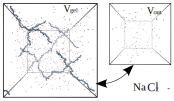
\includegraphics[width=0.7\textwidth]{{figures/simgibbs}.pdf}\caption{Diamond-like network in the simulation box. Color code represents
the individual ion types (red: $\na$, blue: $\cl$, yellow: $\ca$)
and the hydrogel (gray: neutral segment ($\AH$), cyan: charged segment
($\A$)). \label{fig:diamond}.}
\end{figure*}

\subsection{Model}

We propose a cascade desalination process to lower supernatant salinity, it is worth to note that we are not limited with this process only.
For this process the gel must be commpressed/decompressed in an \emph{open} and \emph{closed} system.

By the \emph{open system} we mean that the gel is in thermodynamic equilibrium with an \textbf{infinite} reservoir of an aqueous solution.
%, such that there are the same ion's chemical potential, the same temperature, and desired pressure difference between the gel and the reservoir. The number of  $\na$ and $\cl$ ions and gel volume $\Vgel$ are allowed to change.

By the \emph{closed system} we mean that the gel is equilibrated with a \textbf{finite} reservoir of an aqueous solution, in this case after equilibration the gel and the reservoir again have the same ions chemical potential, the same temperature, and desired pressure difference between the gel and the reservoir. 
Although, the number of ions and volume of gel and reservoir may vary, the total number of ions and the total volume are constant.

The compression of the gel in the \emph{open system} does not affect the salinity in the 
reservoir, thus the density of ions and their chemical potential outside the gel remains constant 
$\cs =$ $\cna=$ $\ccl=$ $\text{Const}$ (\reffig{fig: open}). 
On the contrary, the compression of the gel in the \emph{closed system} changes the salinity in the reservoir, but the total number of $\na$ and $\cl$ ions in the gel and in the reservoir, \ie in the volume $\Vbox$ (\reffig{fig: closed}), remains constant.

In the both cases there is two coexisting systems with constant $\mu P T$ allowed to exchange particles and change volume, which is represented as Gibbs ensemble.


Unfortunately, there is no universal computationally effective technique to sample pressure difference, volume, and number of particles at the same. To equilibrate and sample pressure difference and volume we use molecular dynamics (MD) simulation, while equlibration and sampling of ions distribution between the gel and a reservoir is done via Monte-Carlo (MC) simulation. In this sence employed techniques is called MCMD. 

To simulate processes in \emph{open system} and  \emph{closed system} two complementary models MC and MD were implemented.

\subsubsection*{Molecular Dynamics model}

Our MD model of the gel is a network of 16 linear polymer chains, each consisting of 30 monomer 
units. 
These polymer chains are connected to a diamond-like network by 8 crosslinking units.
This means, there are $\Ngel=16\cdot30 + 8=488$ gel monomers in the simulation box 
(see \reffig{fig:diamond}).
Each monomer unit of the network carries a negative elementary electric charge, thus 
simulating fully ionized polyacidic gel.
Except the particles in the network, the monovalent co- and counter-ions ions, 
$\cl$ and $\na$, are present in simulation box. 
The total electric charge of all the particles in the box is zero, therefore the amount 
of $\na$ ions is bigger than that of $\cl$ by the number of hydrogel units.
The entire simulation box setup employs periodic boundaries.
Coloumb interaction computed by P3M method.
This model is used in MD part of \emph{open system} and \emph{closed system} simulation.

For the MD part of \emph{closed system} simulation analougous simulation box is created without any polymer monomers to model the finite reservoir. 
The amount of $\na$ ions is equal to $\cl$.

By integration Langevin motion equation by Verlet algorithm for each particles we sample 
total energy of the system and pressure. 
Kinetic energy, bonded, non-bonded and Coloumb interaction contribute to the total energy of a system.
Pressure in the system calculated as in ref [Essmann et al., 1995, doi:10.1063/1.470117]
\todo{I do not know if it is needed, ML}

When computing MD the gel and reservoir box are essentially NVT-ensembles.

\subsubsection*{Monte Carlo model}

In the \emph{open system} system box with the gel and the monovalent co- and counter-ions ions, 
$\cl$ and $\na$ is allowed to exchange particles with infinite reservoir with constant chemical potential.


\dots


In the \emph{closed system} system two boxes one with the gel and the other with ions pairs only iare allowed to exchange particles.


\begin{figure*}[h]
\centering 
\subfloat[Open system \label{fig: open}]
{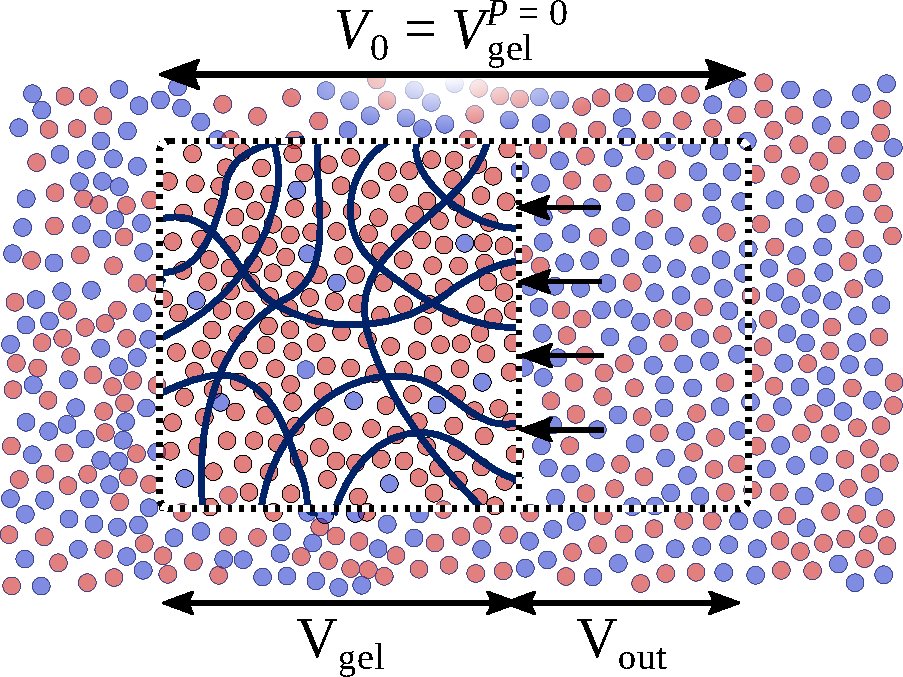
\includegraphics[width=0.5\textwidth]{figures/gc.pdf}}
\subfloat[Closed system \label{fig: closed}]
{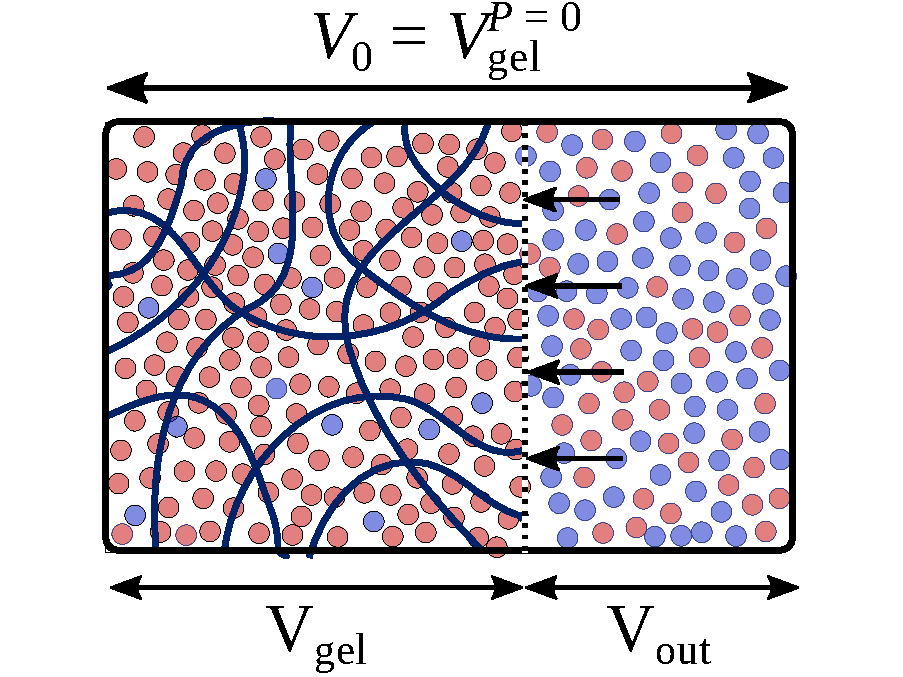
\includegraphics[width=0.5\textwidth]{figures/gibbs.pdf}}
\caption{Diamond-like network in the simulation box. Color code represents
the individual ion types (red: $\na$, blue: $\cl$, yellow: $\ca$)
and the hydrogel (grey: neutral segment ($\AH$), cyan: charged segment
($\A$)). \label{fig:open and closed}.}
\end{figure*}

\subsection{}

\subsection{Gibbs ensemble}
\todo{We have the "Gibbs ensemble" in the title, and this term is not used in the manuscript at all.}
TODO concise description of Gibbs ensemble, solving the task to Reviewer 2, Q5 and Q7

The simulation of the gel compression is performed in two ensembles:
\begin{enumerate}
\item \emph{open system}, when the simulation box with gel exchanges ions with an infinite 
reservoir containing aqueous solution of constant salinity, $\cs$. 
\item emph{closed system}, when the simulation box with the gel exchanges ions with a finite volume of aqueous solution.
\end{enumerate}
The compression of the gel in the \emph{open system} does not affect the salinity in the 
reservoir, thus the density of ions outside the gel remains constant 
$\cs =$ $\cna=$ $\ccl=$ $\text{Const}$ (\reffig{fig: open}). 
On the contrary, the compression of the gel in the \emph{closed system} changes the salinity in the reservoir, but the total number of $\na$ and $\cl$ ions in the gel and in the reservoir, \ie in the volume $\Vbox$ (\reffig{fig: closed}), remains constant.



The amount of the individual ion types in gel, $N_i$, is given by
\begin{equation}
N_i = N_i\gel + \cs\cdot(\Vbox - \Vgel)
\end{equation}
where $i \in \{\na, \cl\}$, $\Vgel$~--- volume of the gel, $\Vbox$~--- the volume in which the gel is compressed. 
$\Vbox$ is the gel volume in the free swelling equilibrium state.


\subsection{Open system}
We use the grand reaction method \cite{Landsgesel2020a,Rud2020} to simulate the open system.
\todo{beter to say "method described in REF", to avoid the word 'grand reaction'}
This method is a hybrid of Molecular dynamics (MD) and Monte Carlo (MC). 
The whole simulation consists of MD and MC subsimulations, consecutively followed one by each other. 
The MD simulation is a standard Langevin dynamics \cite{Grest1986}, which models the mechanical motion of all particles in the system. 
MC simulates the thermodynamic equilibrium with reservoir and handles the ion exchange with the simulation box. 
The insertion (and deletion) of ion pairs is considered as a reaction of creation (or annihilation) of an ion pair 
\begin{equation}
\varnothing\stackrel{K}{\leftrightarrows}\na+\cl
\end{equation}
with a reaction constant defined by the chemical potential of ions,
$K=\exp\left(\muna+\mucl\right).$
The simulation setup is sketched in \reffig{fig:open}\todo{it is not a 'simulation' setup}.

\subsection{Closed system}
Analogical scheme is used for the simulation of the gel in the closed system. 
The procedure  again consists of subsequent MD and MC subsimulation, but now the MD is running in two simulation boxes simultaneously.
The first box of the volume $\Vgel$ contains the gel with ions and the second box of the volume $\Vout$ contains only ions. 
The total volume of both boxes is constant, $\Vbox=V_{\mathrm{gel}}+V_{\mathrm{out}}$, so the gel compression implies the decrease of $\Vgel$ and increase of $\Vout$.
The simulation setup is sketched in \reffig{fig:closed}. 

\subsection{Algorithm}
The thermodynamic equilibrium between the two subvolumes implies the exchange of ion pairs 
between them.
This is performed by means of MC procedure in a way similar to described in \cite{Panagiotopoulos1988b}.

As mentioned above, the simulation consists of MD and MC subsimulations. The algorithm is following:
\begin{enumerate}
\item Simulate MD in both boxes and collect the observables (pressure, $P$)
\item Perform MC procedure simulating ion exchange and collect the observables (number of ions in both boxes, 
%$\nna\gel$,
$\Ncl\gel$ 
%$\nna\out$ 
and $\Ncl\out$ )
\item Repeat the procedure until the desired length of sample arrays is reached.
\end{enumerate}

\section{Results and discussion}

\subsection{Compression in open system}
\begin{figure*}[h]
	\begin{adjustwidth}{-\extralength}{0cm}
	\subfloat[The gel partial pressure vs gel molar volume \label{fig: PV}]
		{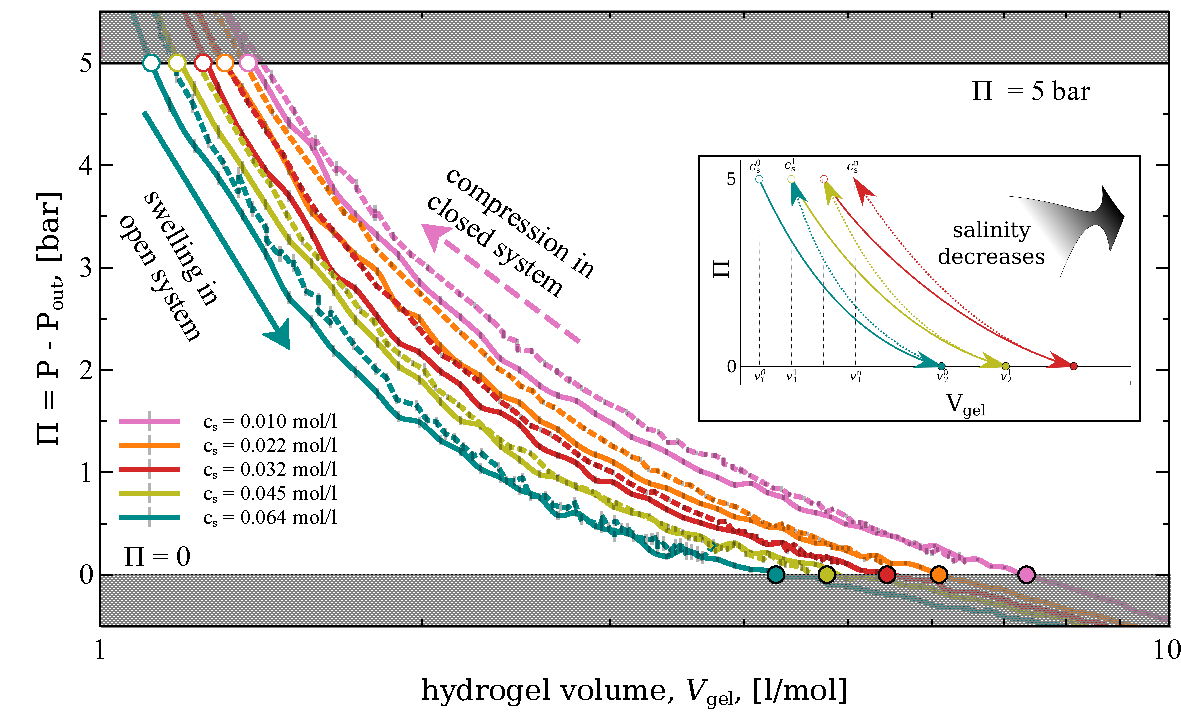
\includegraphics[width=0.65\textwidth]{figures/fig_PV_pub.pdf}}
	\hspace{0.02\textwidth}
	\subfloat[Supernate salinity vs gel molar volume\label{fig: CV}]
		{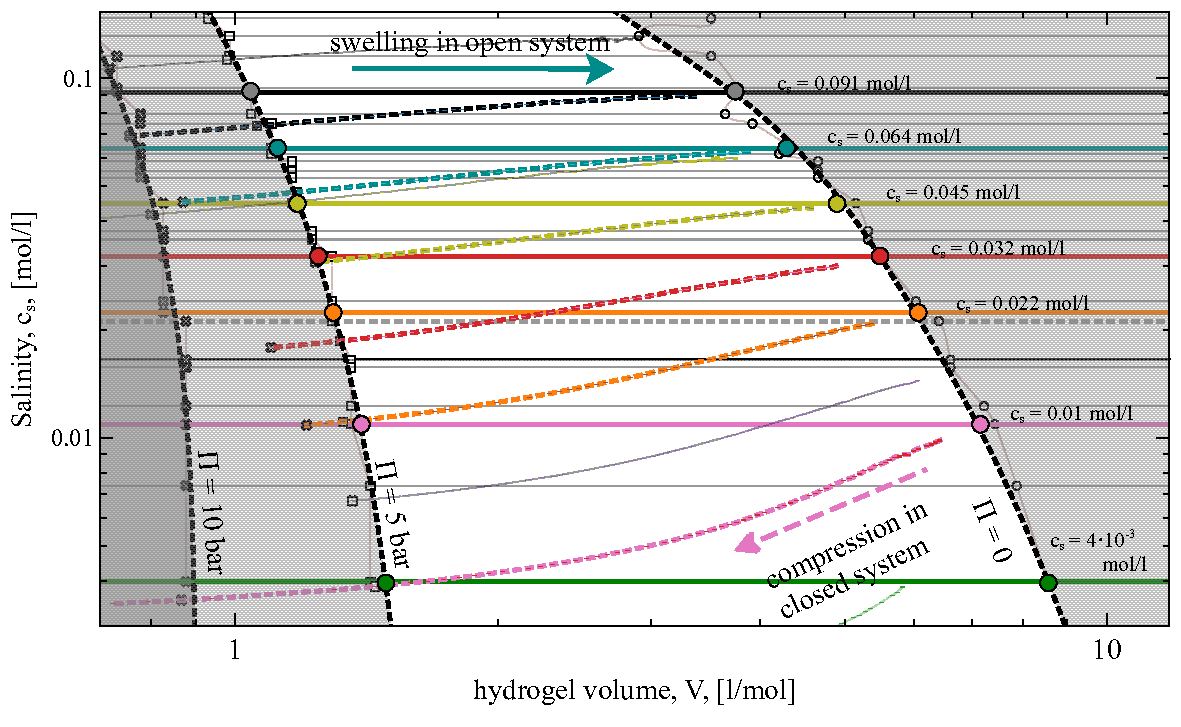
\includegraphics[width=0.65\textwidth]{figures/fig_CV_pub.pdf}}
	\caption{
	The compression of the gel in the \emph{open system} (solid lines) and in the \emph{closed system} (dotted lines). 
	Each solid curve corresponds to different salinity of the reservoir $\cs$ (see legend).
	The shadowed areas limit the states with applied pressure below zero and above 5 bar.\label{fig: PV and CV}}
	\end{adjustwidth}
\end{figure*}
First, we run a set of simulations modeling the gel compression in \emph{open system}, \ie in equilibrium with a big bath of certain salinity, $\cs$. 
The simulations were run for a set of different simulation box volumes. 
Each simulation returned the averaged values of pressure, $P$, and the number of $\cl$ ions, present in the simulation box, $\ncl$. 

In order to get the partial pressure of the gel, we subtracted from $P$ the osmotic pressure of ions in the reservoir: $\Pgel=P - \Pout$.
$\Pout$, in turn, we obtained from a separate simulation of a reservoir, containing ionic gas in equilibrium with the bath of the same salinity $\cs$. 
The gel partial pressure, $\Pgel$, is the pressure that needs to be applied to the gel via a solvent permeable filter to compress the gel to a specific molar volume, $\Vgel$. $\Vgel$ is the gel volume per one mole of gel monomer units.

These dependencies of $\Pgel$ on $\Vgel$ for \emph{open system} for a set of various salinities are presented
in Figure \ref{fig: PV} by solid lines. 
For example, the blue solid line illustrates the compression (or swelling) of the gel in equilibrium with a reservoir of salinity, $\cs=0.063$ mol/l. 
The points where the pressure equals zero, $\Pgel=0$, (indicated by filled circles) are the gel \emph{free swelling equilibrium} states.
These states are characterized by the corresponding molar volume of the gel, $\Vgel^0$ and the amount of ions in gel \{$\Nna^0$, $\Ncl^0$\} 
(Index ``0'' stands for zero bar applied pressure).
The \emph{free swelling equilibrium} states' positions shift towards smaller volumes with increase of salinity. 
In general, the increase of salinity shifts all the $\Pgel(V)$ curves towards smaller volumes.
This effect is well known and is typical for all branched \emph{strong} polyelectrolytes. 
It is caused by the decrease of ions osmotic pressure and by a screening of electrostatic interactions \cite{Zhulina2000, Landsgesel2020a}.
(The salinity dependence of the size of \emph{weak} polyelectrolyte gel is in general non-monotonic. We discuss this case in \cite{Rud2018}.)

\begin{figure*}[h]
\begin{adjustwidth}{-\extralength}{0cm}
\subfloat[Pressure vs gel molar volume \label{fig: NV}]
{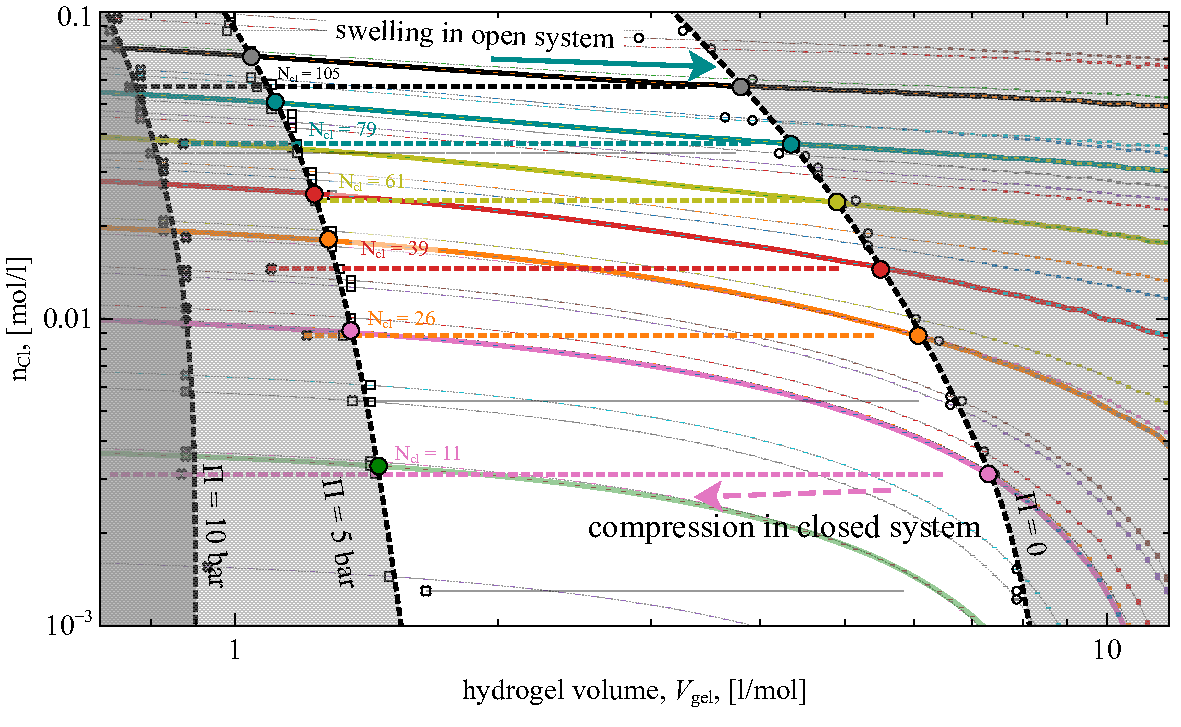
\includegraphics[width=0.65\textwidth]{figures/fig_NV_pub.pdf}}
\hspace{0.02\textwidth}
\subfloat[Salinity vs gel molar volume\label{fig: CN}]
{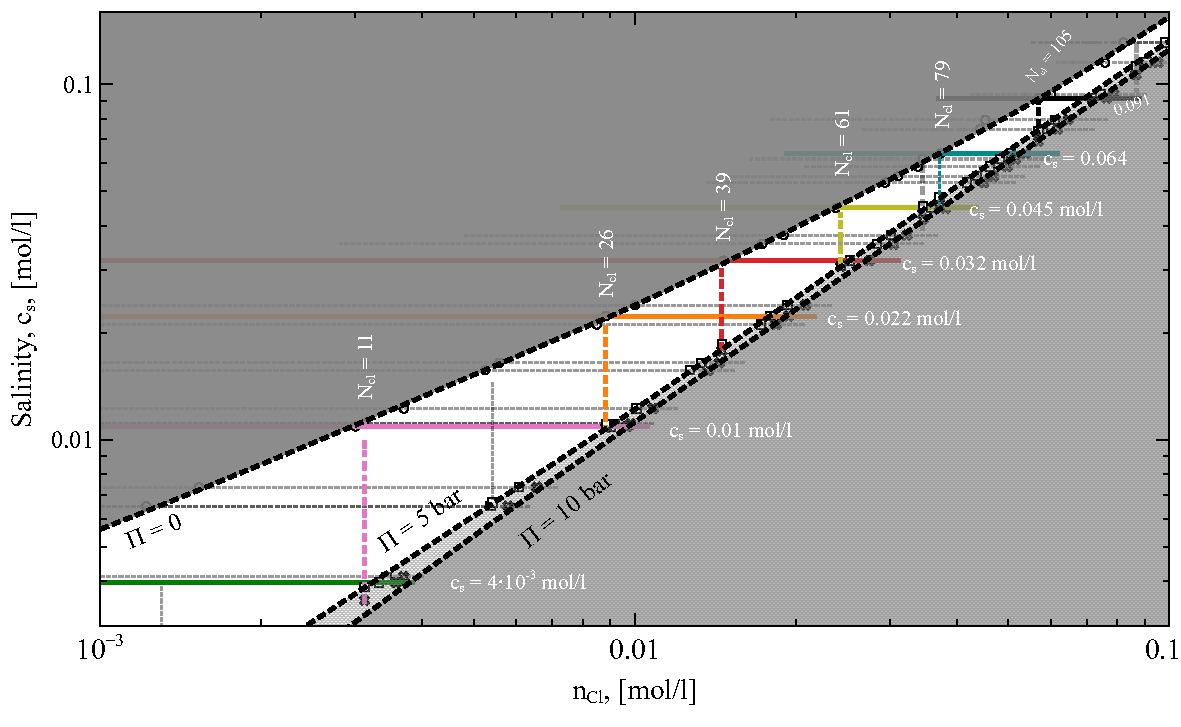
\includegraphics[width=0.65\textwidth]{figures/fig_NVbox_mu_pub.pdf}}
\caption{The compression of the gel in \emph{open system} (solid lines) and in \emph{closed system} (dotted lines). 
Shadowed area limit the states with applied pressure below zero and above 5 bar.
The values $N_\cl$ are the virtual numbers of present $\cl$ ions in \emph{closed system} simulation boxes.
\label{fig: NV and CN}}
\end{adjustwidth}
%\todoi{Replace y-axis labels by $\ncl$}
\end{figure*}

\subsection{Compression in closed system}
The simulations in \emph{closed systems} start from the $\Vgel^0$ and \{$\Nna^0$, $\Ncl^0$\} values
obtained from the corresponding \emph{open system} simulations.
The simulation of gel compression in a closed volume, $\Vbox$, starts at the point $\Vbox = \Vgel^0$,
and ion content $\Ncl^0$ for $\cl$ ions. The $\na$ ions amount is neutralize the system, $\Nna^0 = $$\Ncl^0 + \Ngel$.

We prepare two systems: one for simulation of the gel at the volume $\Vgel$,
and the other one for simulation of the supernatant solution at the volume $\Vout = \Vbox - \Vgel$.
Note that the ions of the amount $\Ncl^0$ and $\Nna^0$ are shared by the two volumes. 

The processes of the gel compression in \emph{closed system} are depicted in Figure~\ref{fig: PV} as dotted lines.
In this plot, for example, the blue dotted line illustrates the compression of the gel equilibrated with the solution of salinity $\cs=0.063$ mol/l at volume, at which the gel has at zero pressure. 
The volume values $\Vgel$ and $\Vout$ are comparable in the \emph{closed system} case.
Therefore, the gel compression causes decrease of the salinity in the supernate, $\cs$. 
This dependence is illustrated in \reffig{fig: CV}, where the same swelling/compression processes are displayed in different coordinates: \ie salinity of supernate versus the gel molar volume, $\cs(\Vgel)$.
In these coordinates, all the open system compressions show up as horizontal lines, which reflects the constant salinity, whereas the compressions in closed system demonstrate the change of $\cs$ from $\cs^{0}=0.063$ at zero pressure $\Pgel$ to $\cs^{5}=0.045$ mol/l at $P\gel=5$ bar (index ``5'' stands for 5 bar). 

Although the salinity during compression in \emph{open system} remains constant, the amount of ions in the compressed subsystem (\ie in the volume where the gel is compressed (or swells)), changes.
Here, the compression volume $\Vbox$ is the volume of the \emph{free swelling equilibrium} state of the gel, $\Vbox = \Vgel^0$.
Figure \ref{fig: NV} shows number of $\cl$ ions in the volume $\Vbox$ per unit volume, $\ncl =$ $\Ncl/\Vbox$, as a function of the gel molar volume. 
The depicted values can be considered as the average density of $\cl$ ions in the compression volume $\Vbox$. 

The $\ncl$-$\Vgel$ dependencies look like horizontal lines in the case of \emph{closed system} compression,
whereas $\ncl$ increases with $\Vgel$ during the compression in the \emph{open system} case. 
This implies, that the compression of the gel in the \emph{open system} pulls out the ions from the bath to the compression volume, $\Vbox$. 
And vice versa, the swelling of the gel pushes ions out to the bath.

Finally, the same processes are depicted in Figure \ref{fig: CN} in coordinates $\ncl$ --- $\cs$. 
In these coordinates, both ways of the compression, in \emph{open} and in \emph{closed} systems, appear as straight vertical and horizontal lines correspondingly. 

In our study, we modeled the compression of the gel in equilibrium with reservoirs of 40 different salinities, ranging from 0.001 to 0.5 mol/l. 
The \emph{open system} compressions resulted in a defined free swelling equilibrium states,
which we used as the initial conditions for the respective compressions in \emph{closed systems}. 
All the corresponding dependencies are depicted in Figures~\ref{fig: PV and CV} and \ref{fig: NV and CN} as thin grey dashed lines (some of them are highlighted and colored).
The states corresponding to $P^{gel}=0$, 5 and 10 bar pressure are marked by open circles, squares, and crosses respectively. 
The non-shadowed areas in the Figures highlight the states in which the gel partial pressure ranges between the experimentally relevant values, 0 and 5 bar.

\subsection{Desalination scheme}
It follows that the compression of the gel in the \emph{closed system} affects the salinity, whereas the compression in the \emph{open system} affects the amount of ions in the gel subsystem. 
Here we show how to employ these phenomena for water desalination. 
The highlighted colored lines on plots of Figures \ref{fig: PV and CV} and \ref{fig: NV and CN} form a sequence gel swellings and compressions, following one by one, correspondingly in \emph{open} and \emph{closed} systems. 
This sequence forms the water desalination process.
Starting from swelling the gel in the \emph{open system} at high salinity ($\cs=0.091$ mol/l, solid black line), the gel is compressed in the \emph{closed system} until the pressure reaches 5 bar (dashed black line). 
Then the same gel swells in a reservoir of a bit lower salinity in the \emph{open system} (\ie $\cs=0.064$ mol/l, light blue line). 
After the swelling, the gel is compressed again with the pressure 5 bar in \emph{closed system} (dashed light blue line).  
Then the gel swells in a reservoir of even smaller salinity ($\cs=0.045$ mol/l, solid yellow line), and so on. 
This chain of alternating swellings and compressions ends up when salinity is equal to $\cs=4\cdot10^{-3}$ mol/l after the compression in the \emph{closed system} (dashed magenta line).

The plots in Figures \ref{fig: PV and CV} and \ref{fig: NV and CN} depict the whole process in all possible coordinate representations.
In all plots, the lines corresponding to sequential swellings and compressions during the whole desalination process resemble a 'pathway'.
In particular, the desalination process depicted in Figure~\ref{fig: CN} resembles a staircase,
where the \emph{open system} processes are horizontal lines and the \emph{closed system} processes are vertical lines.

%\begin{enumerate}
%    \item as gel partial pressure versus gel molar volume, $\Pgel(\Vgel)$ (\ref{fig: PV}), 
%    \item as supernatant salinity versus gel molar volume, $\cs(\Vgel)$ (\ref{fig: CV}),
%    \item the amount of $\cl$ ions in a compression volume versus gel volume, $\ncl(\Vgel)$ (\ref{fig: NV}), 
%    \item $\ncl$ as function of supernatant salinity.
%\end{enumerate}




%Then we repeat the simulation of hydrogel swelling in open system but setting as a salinity of the reservoir the new, obtained from the previous process, value $\cs=$ 0.045 mol/l. 
%Again, as soon as we obtain the free swelling equilibrium state (at new salinity), with corresponding new values of $V\gel$ and $\ncl$, we start simulating the compression in closed system. Now the salinity changes again, decreasing from 0.045 to 0.031 mol/l (at 5 bar). 
%These two processes are depicted by solid and dotted yellow lines in Figure~\ref{fig:fig_PV}.
%The Figure shows also the repetition of this procedure three more times until the salinity reaches the value $\cs=0.01$ mol/l. 
%The last dashed magenta line shows the compression in closed system which ends up with $\cs=4\cdot10^{-4}$ mol/l. 
%Schematically this process is depicted in the inset to the plot.



%The same process is depicted on Figure~\ref{fig:fig_CV} but in different coordinates: salinity versus volume. 
%In this coordinates the swelling in open system appear to be horizontal line, since the salinity in this process is constant. 
%Again we start from swelling in open system untill the gel reaches its free swelling equilibrium (solid blue line).
%Then the gel is compressed in closed system (dashed blue line), ending up in a state with applied to the gel pressure 5 bar. 
%In this process the surrounding solution salinitiy changes from 0.064 to 0.045 mol/l.
%Then the gel again swells in open system, but at new salinity. 

\subsection{The efficiency of desalination}
The theoretical minimum specific energy for seawater desalination (
%$\cs=35$ g/l, 
$\cs\simeq0.6$ mol/l as for pure NaCl) is $\sim3.9$ kJ/l (1.1 kWh/m$^3$) for 50\% recovery \cite{Wang_2020}.
This value is calculated as follows 
\begin{equation}
W=2RT\left(\frac{c_{f}}{R_{w}}\ln\frac{c_{b}}{c_{f}}-c_{p}\ln\frac{c_{b}}{c_{p}}\right)
\label{eq:SEC}
\end{equation}
where $R$ is a universal gas constant, $c_{f}$ is the salinity of feed water, $c_p$ is the salinity of product water and $c_b$ is the salinity of the brine, which necessarily appears in any desalination process. 
$R_{w}$ is a recovery ratio, \ie the ratio between volume of produced water and the volume of the feed water. 
50\% recovery ratio means that one part of feed water divides into two equal volume solutions of the product water and of the brine.
Of course, a significant amount of additional energy is required to operate the system\cite{Kim_2019}. 
It has been reported that the specific energy consumption (SEC) of reverse osmosis (RO) process is 2.5~-- 4.0 kWh/m3 (9~-- 14.4 kJ/l), which is significantly higher than its minimum specific energy.
The SEC of a real-scale RO plant is even higher, approximately 3.5~-- 4.5 kWh/$m^{3}$ (12.6 - 16.2 kJ/L), including pre-treatment and post-treatment processes \cite{Kim_2018}. 
%Because of the inherent high energy requirement for RO desalination, seawater is not commonly utilized over traditional surface water.

In order to compare the efficiency of the process presented in \ref{fig: PV and CV} and \ref{fig: NV and CN} with provided values, we collect the corresponding data to the Table~\ref{tab: table}.
The presented desalination process is a cascade of six swellings in open system, at six different (constant) salinities $\cs$, each followed by six compressions in closed system, at six different (constant) $\ncl$.
Each swelling and compression process is presented as a row of Table~\ref{tab: table}, which is colored by matching the lines in the Figures.
The first column of the table contains values $\cs^0$ and $\cs^5$, which stand for the supernate salinity at 0 and 5 bar compression; in open system, supernate salinity does not change, so $\cs^0$ and $\cs^5$ are presented by a single number. 
The second column contains values of $n^0$ and $n^5$, which stand for the number of $\cl$ ions in compression volume $\Vbox$, at 0 and 5 bar pressure (divided by $\Vbox$). 
The number of ion does not change in closed system compression, thus $n^0$ and $n^5$ are the same in the corresponding rows.
The third column shows the change of the gel volume in corresponding process, $\Delta v$. 
The fourth column contains the work needed for the compression in the corresponding process 
per volume of extracted solution. 
This value is an integral of corresponding $\Pgel(\Vgel)$ dependence \citep{Atkins} 
\begin{equation}
    W = \frac{\int_{v^0}^{v^5} \Pgel d\Vgel}{\Delta v}
\end{equation}
\todo{the equation must be supported by referrence}
Here, in the table, we present the absolute values of the work, 
whereas one should keep in mind that the compression implies the work 
is done by external force and the swelling implies that the work is done by gel.

\begin{table}
\caption{The estimates of the efficiency of the desalination process. All the units are calculated per one mol of gel segments. Values in brackets
are the estimates corresponding to crossection of 'red' and 'orange' lines on the plots of Figures \ref{fig: PV and CV} and \ref{fig: NV and CN}
\label{tab: table}}
\begin{adjustwidth}{-0.0\extralength}{0cm}
		\newcolumntype{C}{>{\centering\arraybackslash}X}
\begin{tabularx}{1\textwidth}{@{\extracolsep{\fill}}ll|lc|c|l|ll}
\multicolumn{1}{l|}{$c_{s}^{0}$, mM} & $c_{s}^{5}$, mM & \multicolumn{1}{l|}{$n_{\cl}^{0}$, mM} & $n_{\cl}^{5}$, mM & $\Delta \Vgel$, l & $|W$\textbar , J/l & \multicolumn{2}{c}{$W^{id}$, J/l}\tabularnewline
\hline 
\hline 
\multirow{2}{*}{{\small{}$91.47$}} & \multirow{2}{*}{} & \multicolumn{2}{l|}{{\small{}$57.08\pm0.122\enskip\longrightarrow$}} & \multirow{2}{*}{{\small{}2.74}} & \multirow{2}{*}{{\small{}$95.4\pm1.9$}} &  & \multirow{2}{*}{}\tabularnewline
 &  & \multicolumn{2}{r|}{{\small{}$71.75\pm0.024$}} &  &  & \multirow{8}{*}{{\small{}\hspace{-1em}}\textcolor{teal}{\small{}$\left.\begin{array}{l}
\\
\\
\\
\\
\\
\\
\\
\\
\end{array}\right\rbrace $$\rotatebox{90}{\hspace{-5em}{\color{teal}\ensuremath{\begin{array}{cc}
W^{\mathrm{sim}}= & 202.8\pm3.2\\
W^{id}= & 52.9\\
R_{w}= & 0.54
\end{array}}}}$}} & \tabularnewline
\cline{1-6} \cline{2-6} \cline{3-6} \cline{4-6} \cline{5-6} \cline{6-6} 
\multicolumn{2}{l|}{{\small{}$89.41\pm0.23\enskip\longrightarrow$}} & \multirow{2}{*}{{\small{}56.90}} & \multirow{2}{*}{} & \multirow{2}{*}{{\small{}2.72}} & \multirow{2}{*}{{\small{}$109.1\pm1.7$}} &  & \multirow{2}{*}{}\tabularnewline
\multicolumn{2}{r|}{{\small{}$73.63\pm0.03$}} &  &  &  &  &  & \tabularnewline
\cline{1-6} \cline{2-6} \cline{3-6} \cline{4-6} \cline{5-6} \cline{6-6} 
\multirow{2}{*}{\textcolor{teal}{\small{}63.93}} & \multirow{2}{*}{} & \multicolumn{2}{l|}{\textcolor{teal}{\small{}$37.28\pm0.08\enskip\longrightarrow$}} & \multirow{2}{*}{\textcolor{teal}{\small{}3.26}} & \multirow{2}{*}{\textcolor{teal}{\small{}$100.9\pm1.7$}} &  & \tabularnewline
 &  & \multicolumn{2}{r|}{\textcolor{teal}{\small{}$50.579\pm0.013$}} &  &  &  & \multirow{8}{*}{{\small{}\hspace{-1em}}\textcolor{olive}{\small{}$\left.\begin{array}{l}
\\
\\
\\
\\
\\
\\
\\
\\
\end{array}\right\rbrace $$\rotatebox{90}{\hspace{-5em}\ensuremath{\begin{array}{cc}
W^{\mathrm{sim}}= & 207.3\pm2.2\\
W^{id}= & 38.2\\
R_{w}= & 0.53
\end{array}}}$}}\tabularnewline
\cline{1-6} \cline{2-6} \cline{3-6} \cline{4-6} \cline{5-6} \cline{6-6} 
\multicolumn{2}{l|}{\textcolor{teal}{\small{}$62.05\pm0.15\enskip\longrightarrow$}} & \multirow{2}{*}{\textcolor{teal}{\small{}37.17}} & \multirow{2}{*}{} & \multirow{2}{*}{\textcolor{teal}{\small{}3.18}} & \multirow{2}{*}{\textcolor{teal}{\small{}$107.4\pm1.4$}} &  & \tabularnewline
\multicolumn{2}{r|}{\textcolor{teal}{\small{}$48.21\pm0.02$}} &  &  &  &  &  & \tabularnewline
\cline{1-6} \cline{2-6} \cline{3-6} \cline{4-6} \cline{5-6} \cline{6-6} 
\multirow{2}{*}{\textcolor{olive}{\small{}44.91}} & \multirow{2}{*}{} & \multicolumn{2}{l|}{\textcolor{olive}{\small{}$23.75\pm0.06\enskip\longrightarrow$}} & \multirow{2}{*}{\textcolor{olive}{\small{}3.82}} & \multirow{2}{*}{\textcolor{olive}{\small{}$106.7\pm1.5$}} &  & \tabularnewline
 &  & \multicolumn{2}{r|}{\textcolor{olive}{\small{}$35.911\pm0.010$}} &  &  & \multirow{8}{*}{{\small{}\hspace{-1em}}\textcolor{red}{\small{}$\left.\begin{array}{l}
\\
\\
\\
\\
\\
\\
\\
\\
\\
\end{array}\right\rbrace \rotatebox{90}{\hspace{-5em}\ensuremath{\begin{array}{cc}
W^{\mathrm{sim}}= & 222.3\pm2.5\\
W^{\mathrm{id}}= & 43.8\ {\color{red}{\scriptstyle (41.0)}}\\
R_{w}= & 0.52\ {\scriptstyle (0.46)}
\end{array}}}$}} & \tabularnewline
\cline{1-6} \cline{2-6} \cline{3-6} \cline{4-6} \cline{5-6} \cline{6-6} 
\multicolumn{2}{l|}{\textcolor{olive}{\small{}$43.46\pm0.12\enskip\longrightarrow$}} & \multirow{2}{*}{\textcolor{olive}{\small{}24.27}} & \multirow{2}{*}{} & \multirow{2}{*}{\textcolor{olive}{\small{}3.91}} & \multirow{2}{*}{\textcolor{olive}{\small{}$106.4\pm1.1$}} &  & \tabularnewline
\multicolumn{2}{r|}{\textcolor{olive}{\small{}$30.795\pm0.008$}} &  &  &  &  &  & \tabularnewline
\cline{1-6} \cline{2-6} \cline{3-6} \cline{4-6} \cline{5-6} \cline{6-6} 
\multirow{2}{*}{\textcolor{red}{\small{}31.93}} & \multirow{2}{*}{} & \multicolumn{2}{l|}{\textcolor{red}{\small{}$14.66\pm0.04\enskip\longrightarrow$}} & \multirow{2}{*}{\textcolor{red}{\small{}4.20}} & \multirow{2}{*}{\textcolor{red}{\small{}$107.9\pm1.4$}} &  & \tabularnewline
 &  & \multicolumn{2}{r|}{\textcolor{red}{\small{}$25.297\pm0.006$}} &  &  &  & \multirow{8}{*}{{\small{}\hspace{-1em}}\textcolor{orange}{\small{}$\left.\begin{array}{l}
\\
\\
\\
\\
\\
\\
\\
\\
\\
\end{array}\right\rbrace \rotatebox{90}{\hspace{-5em}\ensuremath{\begin{array}{cc}
W^{\mathrm{sim}}= & 218.7\pm2.2\\
W^{id}= & 66.6\ {\scriptstyle (22.0)}\\
R_{w}= & 0.53\ {\scriptstyle (0.49)}
\end{array}}}$}}\tabularnewline
\cline{1-6} \cline{2-6} \cline{3-6} \cline{4-6} \cline{5-6} \cline{6-6} 
\multicolumn{2}{l|}{\textcolor{red}{\small{}$30.03\pm0.08\enskip\longrightarrow$}} & \multirow{2}{*}{\textcolor{red}{\small{}14.55}} & \multirow{2}{*}{} & \multirow{2}{*}{\textcolor{red}{\small{}$\begin{array}{c}
4.17\\
{\scriptstyle (3.22)}
\end{array}$}} & \multirow{2}{*}{\textcolor{red}{\small{}$\begin{array}{c}
115.6\pm0.9\\
{\scriptstyle (57.3)}
\end{array}$}} &  & \tabularnewline
\multicolumn{2}{r|}{\textcolor{red}{\small{}$\begin{array}{c}
18.585\pm0.004\,\\
{\scriptstyle (22.32)}
\end{array}$}} &  &  &  &  &  & \tabularnewline
\cline{1-6} \cline{2-6} \cline{3-6} \cline{4-6} \cline{5-6} \cline{6-6} 
\multirow{2}{*}{\textcolor{orange}{\small{}22.30}} & \multirow{2}{*}{} & \multicolumn{2}{l|}{\textcolor{orange}{\small{}$8.84\pm0.03\enskip\longrightarrow$}} & \multirow{2}{*}{\textcolor{orange}{\small{}$\begin{array}{c}
4.75\\
{\scriptstyle (3.76)}
\end{array}$}} & \multirow{2}{*}{\textcolor{orange}{\small{}$\begin{array}{c}
108.1\pm1.3\\
{\scriptstyle (68.3)}
\end{array}$}} &  & \tabularnewline
 &  & \multicolumn{2}{r|}{\textcolor{orange}{\small{}$\begin{array}{c}
\text{17.945}\pm\text{0.004}\\
{\scriptstyle (14.56)}
\end{array}$}} &  &  & \multirow{7}{*}{{\small{}\hspace{-1em}}\textcolor{magenta}{\small{}$\left.\begin{array}{l}
\\
\\
\\
\\
\\
\\
\\
\end{array}\right\rbrace \rotatebox{90}{\hspace{-5em}\ensuremath{\begin{array}{cc}
W^{\mathrm{sim}}= & 227.5\pm2.3\\
W^{id}= & 69.7\\
R_{w}= & 0.55
\end{array}}}$}} & \tabularnewline
\cline{1-6} \cline{2-6} \cline{3-6} \cline{4-6} \cline{5-6} \cline{6-6} 
\multicolumn{2}{l|}{\textcolor{orange}{\small{}$20.74\pm0.06\enskip\longrightarrow$}} & \multirow{2}{*}{\textcolor{orange}{\small{}8.83}} & \multirow{2}{*}{} & \multirow{2}{*}{\textcolor{orange}{\small{}$4.71$}} & \multirow{2}{*}{\textcolor{orange}{\small{}$110.8\pm0.8$}} &  & \tabularnewline
\multicolumn{2}{r|}{\textcolor{orange}{\small{}$11.082\pm0.002$}} &  &  &  &  &  & \tabularnewline
\cline{1-6} \cline{2-6} \cline{3-6} \cline{4-6} \cline{5-6} \cline{6-6} 
\multirow{2}{*}{\textcolor{magenta}{\small{}10.90}} & \multirow{2}{*}{} & \multicolumn{2}{l|}{\textcolor{magenta}{\small{}$3.00\pm0.01\enskip\longrightarrow$}} & \multirow{2}{*}{\textcolor{magenta}{\small{}6.08}} & \multirow{2}{*}{\textcolor{magenta}{\small{}$106.9\pm1.1$}} &  & \tabularnewline
 &  & \multicolumn{2}{r|}{\textcolor{magenta}{\small{}9.011$\pm$0.002}} &  &  &  & \tabularnewline
\cline{1-6} \cline{2-6} \cline{3-6} \cline{4-6} \cline{5-6} \cline{6-6} 
\multicolumn{2}{l|}{\textcolor{magenta}{\small{}$9.83\pm0.05\enskip\longrightarrow$}} & \multirow{2}{*}{\textcolor{magenta}{\small{}3.12}} & \multirow{2}{*}{} & \multirow{2}{*}{\textcolor{magenta}{\small{}5.78}} & \multirow{2}{*}{\textcolor{magenta}{\small{}$119.4\pm1.0$}} &  & \tabularnewline
\multicolumn{2}{r|}{\textcolor{magenta}{\small{}$3.862\pm0.001$}} &  &  &  &  &  & \tabularnewline
\end{tabularx}
\end{adjustwidth}
\end{table}

To give a clue of comparison with ideal desalination process efficiency, the fifth column provides the values of specific energy consumption, $W^\text{id}$, which are calculated by means of \refeq{eq:SEC}, using the following procedure:
Let§s assume the concentration of the feed solution to be $\cs^f=44.91$ mmol/l and the concentrations of product and brine solutions to be $\cs^p=31.93$ mmol/l and $\cs^b = 63.93$ mmol/l, respectively.
\begin{enumerate}
    \item The gel, equilibrated with the feed solution, is compressed in the \emph{closed system}.
    The gel volume decreases by $\Delta v^p = 3.69$ liters and the salinity of supernate decreases from $\cs^f$ to $\cs^p$.
    The volume of the product solution is $\Delta v^p$
    \item The squeezed gel is put back into the feed solution and is quilibrated there under pressure, so it does not swell. 
    \item After the equilibration, the gel swells in the \emph{closed system} and the salinity of the external solution increases to the value $\cs^b$.
    \item Finally, the gel is taken out and compressed by 5 bar in the \emph{open system} in equilibrium with the brine bath. 
    The change of the gel volume in this process is $\Delta v^b = 3.26$ l/mol, which equals to the volume of the produced brine. 
\end{enumerate}
Thus the recovery ratio $R_w = \Delta v^p / (\Delta v^p + \Delta v^b) \simeq $ 0.53 and the theoretical minimum specific energy of the desalination process with corresponding $\cs^f$, $\cs^p$ and $\cs^b$ is $W^{id} =$ 38.2 J/l (\refeq{eq:SEC}).

The estimated $W^{id}$ values are provided in the fifth column of the table, for five triplets of $\cs^f$, $\cs^p$,$\cs^b$ values .
$W_{\mathrm{sim}}$ is the energy calculated by integration of $\Pgel(\Vgel)$ dependencies as the sum of corresponding compressions in \emph{closed} and \emph{open} systems, $W_{\mathrm{id}}$ is the estimation based on the equation \refeq{eq:SEC} and $R_w$ is the corresponding recovery ratio.
\todo{how the integration was performed}
Note that calculating the $W_{\mathrm{sim}}$ we accounted for only the work done on the gel during the compression, whereas the work done by the gel itself during swelling was not taken into account.
The ratio between $W_{\mathrm{sim}}$ and $W_{\mathrm{id}}$ ranges from 3.26 to 5.43, which is comparable to that of RO.

\subsection{Study limitations}
Like other simulation based studies, our research has a limited validity,
primarily resulting from the simplifications applied in the used model.
For example, our coarse-grained model cannot differentiate polystyrene sulphonate gel from other strong polyacidic gels.
However, these limitations are also the advantage of our model because the results of our study
can be applied to similar systems, including polybasic gels with all the charges reversed.

\subsection{Implications and future perspectives}
We are aware that the concept introduced in this simulation study need to be experimentally verified.


\section{Conclusions}
We have modeled the compression of the gel in thermodynamic equilibrium with the reservoir of the limited water amount.
We have shown that the compression always decreases the surrounding salinity in the case of strong polyelectrolyte gel.
We have modeled the process of water desalination by sequential combinations of two processes: 
(1) swelling of the gel in \emph{open system}, exchanging ions with a big reservoir at constant salinity
(2) compression of the gel in \emph{closed system}, when the gel affects the salinity in the surrounding solution
We estimated the energy consumption of the whole process for producing a liter of potable water from brine as $W^{id} =$ 38.2 J/l.
Let us compare this value with the energy cost of RO, which is around 20000 J/l.
We have shown that the propsed gel compression method can compete with modern technologies used in modern industry.



%%%%%%%%%%%%%%%%%%%%%%%%%%%%%%%%%%%%%%%%%%
\vspace{6pt} 

%%%%%%%%%%%%%%%%%%%%%%%%%%%%%%%%%%%%%%%%%%
%% optional
%\supplementary{The following supporting information can be downloaded at:  \linksupplementary{s1}, Figure S1: title; Table S1: title; Video S1: title.}

% Only for the journal Methods and Protocols:
% If you wish to submit a video article, please do so with any other supplementary material.
% \supplementary{The following supporting information can be downloaded at: \linksupplementary{s1}, Figure S1: title; Table S1: title; Video S1: title. A supporting video article is available at doi: link.}

%%%%%%%%%%%%%%%%%%%%%%%%%%%%%%%%%%%%%%%%%%
\authorcontributions{Conceptualization, O.R. ; methodology, M.L.; software, M.L.; validation, M.L., L.N. and O.R.; formal analysis, L.N.; data curation, M.L.; writing---original draft preparation, O.R.; writing---review and editing, L.N. 
%All authors have read and agreed to the published version of the manuscript.', please turn to the  \href{http://img.mdpi.org/data/contributor-role-instruction.pdf}{CRediT taxonomy} for the term explanation. Authorship must be limited to those who have contributed substantially to the work~reported.
}

\funding{``This research was funded by Czech Science Foundation grant number 19-17847Y'' and Government of Russian Federation  grant number 14.W03.31.0022. }

\acknowledgments{This research was supported by the Czech Science Foundation (grant 19-17847Y)
Government of Russian Federation, grant number 14.W03.31.0022. 
}

\conflictsofinterest{The authors declare no conflict of interest.} 

%%%%%%%%%%%%%%%%%%%%%%%%%%%%%%%%%%%%%%%%%%
\begin{adjustwidth}{-\extralength}{0cm}
%\printendnotes[custom] % Un-comment to print a list of endnotes

\reftitle{References}

% Please provide either the correct journal abbreviation (e.g. according to the “List of Title Word Abbreviations” http://www.issn.org/services/online-services/access-to-the-ltwa/) or the full name of the journal.
% Citations and References in Supplementary files are permitted provided that they also appear in the reference list here. 

%=====================================
% References, variant A: external bibliography
%=====================================
%\bibliography{your_external_BibTeX_file}
\bibliography{lit/gibbs}


% If authors have biography, please use the format below
%\section*{Short Biography of Authors}
%\bio
%{\raisebox{-0.35cm}{\includegraphics[width=3.5cm,height=5.3cm,clip,keepaspectratio]{Definitions/author1.pdf}}}
%{\textbf{Firstname Lastname} Biography of first author}
%
%\bio
%{\raisebox{-0.35cm}{\includegraphics[width=3.5cm,height=5.3cm,clip,keepaspectratio]{Definitions/author2.jpg}}}
%{\textbf{Firstname Lastname} Biography of second author}

% For the MDPI journals use author-date citation, please follow the formatting guidelines on http://www.mdpi.com/authors/references
% To cite two works by the same author: \citeauthor{ref-journal-1a} (\citeyear{ref-journal-1a}, \citeyear{ref-journal-1b}). This produces: Whittaker (1967, 1975)
% To cite two works by the same author with specific pages: \citeauthor{ref-journal-3a} (\citeyear{ref-journal-3a}, p. 328; \citeyear{ref-journal-3b}, p.475). This produces: Wong (1999, p. 328; 2000, p. 475)

%%%%%%%%%%%%%%%%%%%%%%%%%%%%%%%%%%%%%%%%%%
%% for journal Sci
%\reviewreports{\\
%Reviewer 1 comments and authors’ response\\
%Reviewer 2 comments and authors’ response\\
%Reviewer 3 comments and authors’ response
%}
%%%%%%%%%%%%%%%%%%%%%%%%%%%%%%%%%%%%%%%%%%
\end{adjustwidth}
\end{document}

